\section*{Graphs}
\begin{itemize}
    \item \textbf{\ul{simple definitions}}
    \begin{itemize}[leftmargin = 1em]
    % \setlength{\itemindent}{-1.5em}
        \item path: sequence of verticies $\{v_1, v_2, \ldots, v_k\}$ s.t there exists an edge between consecutive vertices 
        \item simple path: a path that doesn't pass through any vertex more than once
        \item cycle: path w/ common beginning and ending (ex. $\{ v_1, v_2, \ldots, v_k \},~ v_1 = v_k$)
    \end{itemize}
    \item \textbf{\ul{types of graphs:}}
    \begin{itemize}[leftmargin = 1em]
    % \setlength{\itemindent}{-1.5em}
        \item simple: no self-edge and multi-edged vertices
        \item cyclic: graph got at least 1 cycle
        \item connected: every pair of distinct vertices has an edge b/t them 
        \item complete: every vertex has an edge to every other vertex in the graph
        \item tree: undirected. connected, acyclic graph 
        %insert some picture if have space
    \end{itemize}
    % \vfill\null \columnbreak
    \item \ul{\textbf{math for graphs}}: let graph $G = (V,E)$, $| V| = n $ and $|E| = m$ 
    \begin{itemize}[leftmargin = 1em]
    % \setlength{\itemindent}{-1.5em}
        \item simple graphs:
        \begin{align*}
            &\text{sum of degrees in G: } \small {\scriptstyle \sum} _{v \in V} deg(v) = 2m \\
            &\text{\# of edges in complete graph: } m = \frac{n}{2} (n-1)
        \end{align*}
        \item connected simple graph: $O(n) \subset O(m) \subset O(n^2)$ \\
        $\longrightarrow m \in O(n) \Longrightarrow $ graph is sparse \\
        $\longrightarrow m \in O(n^2) \Longrightarrow$ graph is dense 
        \item min \# of edges in connected graph: $m = n-1$
        \item max \# of edges in connected graph\\
        $\longrightarrow$ simple: $n(n-1)/2$ (complete graph)\\
        $\longrightarrow$ not simple: DNE
    \end{itemize} 
    \item topological ordering: all vertices line up in a way that all edges point forward (top. ordering might not be unique)
    % \item DAG: directed acyclic graph 
    % $\longrightarrow G$ is a DAG if it has a topological ordering ($\therefore$ DAG means no cycles
    \item \ul{\textbf{some propositions:}}
    \begin{itemize}[leftmargin = 1em]
    % \setlength{\itemindent}{-1.5em}
        \item any pair of v's in a \ul{tree}, there's a path that connects them
        \item any graph w/ n vertices and n edges has a cycle
        \item let $G$ be an undirected graph w/ $n$ vertices, if any of the following 2 is True, all 3 is True
        \begin{enumerate}
            \item G is connected
            \item G is acyclic
            \item G has $n-1$ edges
        \end{enumerate}
    \end{itemize}
    \item basic graph function runtime\\
        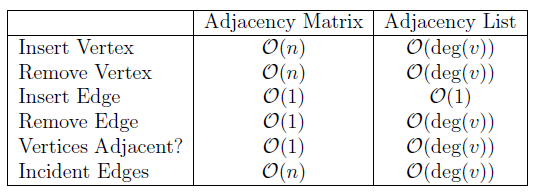
\includegraphics[scale = 0.8]{pictures/runtime graph basic.png} 
\end{itemize}
% \newpage
\subsection*{Search Algorithm}
\begin{itemize}
    \item \ul{\textbf{runtime for graph searching algorithms}} \\
    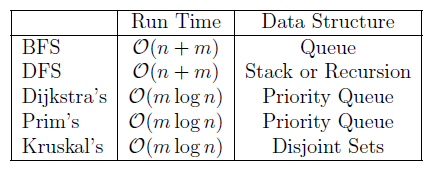
\includegraphics[scale = 0.9]{pictures/runtime graph algo.png}
    \item Prim's and Krushkal's are used to find MST in a weighted graph (can handle negative edges)
    \item Dijkstra's used to find shortest path between two nodes in a weighted graph (cannot handle negative edges)
    \item \textbf{Note}: heights of BFS \& DFS nodes depends on start node and order nodes are checked
    \vfill\null \columnbreak
    \item BFS
    \begin{itemize}[leftmargin = 1em]
        \item uses a queue $\rightarrow$ explores the graph in layers
        \item used to find the shortest path from $s$ to all $v \in V$
    \end{itemize}
    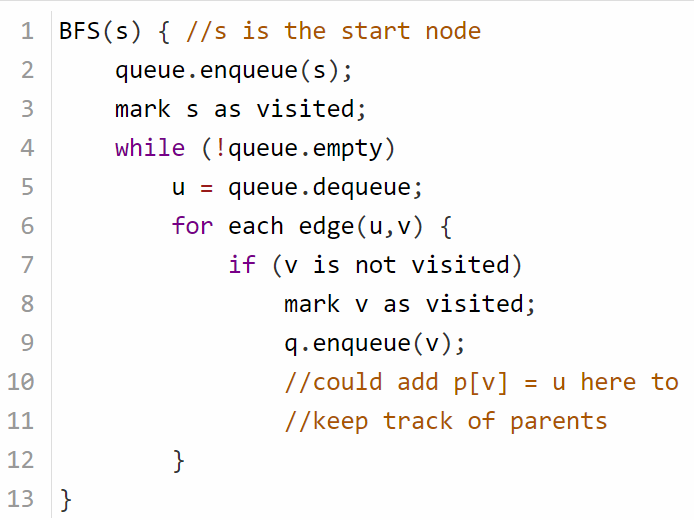
\includegraphics[scale = 0.6]{pictures/BFS code.png} 
    \item DFS
    \begin{itemize}[leftmargin = 1em]
        \item uses a stack/recursion
        \item explores the point further from the graph first
        \item does not find the shortest path 
        \item can identify cycles
    \end{itemize}
    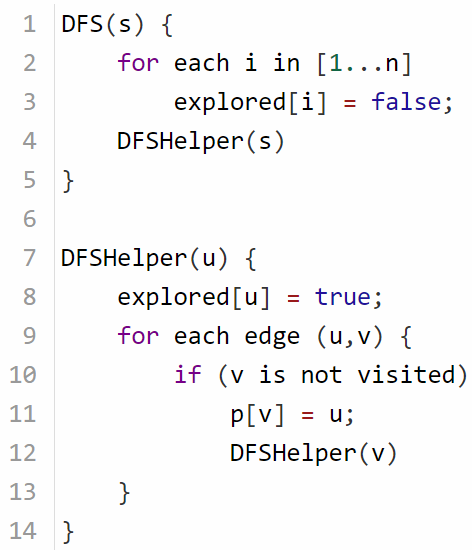
\includegraphics[scale = 0.6]{pictures/DFS code.png}
   
\end{itemize}
